% Created by tikzDevice version 0.12.6 on 2025-04-07 20:16:07
% !TEX encoding = UTF-8 Unicode
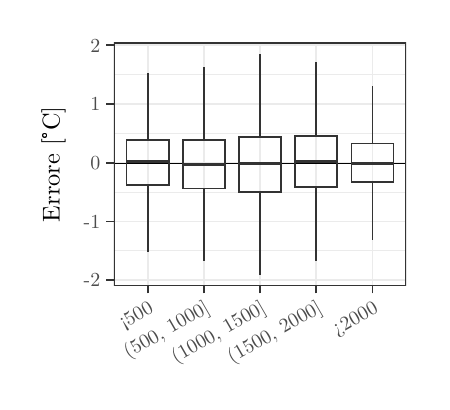
\begin{tikzpicture}[x=1pt,y=1pt]
\definecolor{fillColor}{RGB}{255,255,255}
\path[use as bounding box,fill=fillColor] (0,0) rectangle (142.26,128.04);
\begin{scope}
\path[clip] (  0.00,  0.00) rectangle (142.26,128.04);
\definecolor{drawColor}{RGB}{255,255,255}

\path[draw=drawColor,line width= 0.6pt,line join=round,line cap=round,fill=fillColor] (  0.00,  0.00) rectangle (142.26,128.04);
\end{scope}
\begin{scope}
\path[clip] ( 31.18, 34.79) rectangle (136.76,122.54);
\definecolor{fillColor}{RGB}{255,255,255}

\path[fill=fillColor] ( 31.18, 34.79) rectangle (136.76,122.54);
\definecolor{drawColor}{gray}{0.92}

\path[draw=drawColor,line width= 0.3pt,line join=round] ( 31.18, 47.41) --
	(136.76, 47.41);

\path[draw=drawColor,line width= 0.3pt,line join=round] ( 31.18, 68.63) --
	(136.76, 68.63);

\path[draw=drawColor,line width= 0.3pt,line join=round] ( 31.18, 89.84) --
	(136.76, 89.84);

\path[draw=drawColor,line width= 0.3pt,line join=round] ( 31.18,111.06) --
	(136.76,111.06);

\path[draw=drawColor,line width= 0.6pt,line join=round] ( 31.18, 36.80) --
	(136.76, 36.80);

\path[draw=drawColor,line width= 0.6pt,line join=round] ( 31.18, 58.02) --
	(136.76, 58.02);

\path[draw=drawColor,line width= 0.6pt,line join=round] ( 31.18, 79.24) --
	(136.76, 79.24);

\path[draw=drawColor,line width= 0.6pt,line join=round] ( 31.18,100.45) --
	(136.76,100.45);

\path[draw=drawColor,line width= 0.6pt,line join=round] ( 31.18,121.67) --
	(136.76,121.67);

\path[draw=drawColor,line width= 0.6pt,line join=round] ( 43.36, 34.79) --
	( 43.36,122.54);

\path[draw=drawColor,line width= 0.6pt,line join=round] ( 63.67, 34.79) --
	( 63.67,122.54);

\path[draw=drawColor,line width= 0.6pt,line join=round] ( 83.97, 34.79) --
	( 83.97,122.54);

\path[draw=drawColor,line width= 0.6pt,line join=round] (104.28, 34.79) --
	(104.28,122.54);

\path[draw=drawColor,line width= 0.6pt,line join=round] (124.58, 34.79) --
	(124.58,122.54);
\definecolor{drawColor}{RGB}{0,0,0}

\path[draw=drawColor,line width= 0.1pt,line join=round] ( 31.18, 79.24) -- (136.76, 79.24);
\definecolor{drawColor}{gray}{0.20}

\path[draw=drawColor,line width= 0.6pt,line join=round] ( 43.36, 87.36) -- ( 43.36,111.63);

\path[draw=drawColor,line width= 0.6pt,line join=round] ( 43.36, 71.17) -- ( 43.36, 46.90);

\path[draw=drawColor,line width= 0.6pt] ( 35.75, 87.36) --
	( 35.75, 71.17) --
	( 50.98, 71.17) --
	( 50.98, 87.36) --
	( 35.75, 87.36) --
	cycle;

\path[draw=drawColor,line width= 1.1pt] ( 35.75, 79.57) -- ( 50.98, 79.57);

\path[draw=drawColor,line width= 0.6pt,line join=round] ( 63.67, 87.47) -- ( 63.67,113.78);

\path[draw=drawColor,line width= 0.6pt,line join=round] ( 63.67, 69.89) -- ( 63.67, 43.61);

\path[draw=drawColor,line width= 0.6pt] ( 56.05, 87.47) --
	( 56.05, 69.89) --
	( 71.28, 69.89) --
	( 71.28, 87.47) --
	( 56.05, 87.47) --
	cycle;

\path[draw=drawColor,line width= 1.1pt] ( 56.05, 78.47) -- ( 71.28, 78.47);

\path[draw=drawColor,line width= 0.6pt,line join=round] ( 83.97, 88.64) -- ( 83.97,118.55);

\path[draw=drawColor,line width= 0.6pt,line join=round] ( 83.97, 68.69) -- ( 83.97, 38.78);

\path[draw=drawColor,line width= 0.6pt] ( 76.36, 88.64) --
	( 76.36, 68.69) --
	( 91.59, 68.69) --
	( 91.59, 88.64) --
	( 76.36, 88.64) --
	cycle;

\path[draw=drawColor,line width= 1.1pt] ( 76.36, 78.95) -- ( 91.59, 78.95);

\path[draw=drawColor,line width= 0.6pt,line join=round] (104.28, 88.85) -- (104.28,115.71);

\path[draw=drawColor,line width= 0.6pt,line join=round] (104.28, 70.56) -- (104.28, 43.57);

\path[draw=drawColor,line width= 0.6pt] ( 96.66, 88.85) --
	( 96.66, 70.56) --
	(111.89, 70.56) --
	(111.89, 88.85) --
	( 96.66, 88.85) --
	cycle;

\path[draw=drawColor,line width= 1.1pt] ( 96.66, 79.54) -- (111.89, 79.54);

\path[draw=drawColor,line width= 0.6pt,line join=round] (124.58, 86.24) -- (124.58,106.88);

\path[draw=drawColor,line width= 0.6pt,line join=round] (124.58, 72.27) -- (124.58, 51.46);

\path[draw=drawColor,line width= 0.6pt] (116.97, 86.24) --
	(116.97, 72.27) --
	(132.20, 72.27) --
	(132.20, 86.24) --
	(116.97, 86.24) --
	cycle;

\path[draw=drawColor,line width= 1.1pt] (116.97, 79.11) -- (132.20, 79.11);

\path[draw=drawColor,line width= 0.6pt,line join=round,line cap=round] ( 31.18, 34.79) rectangle (136.76,122.54);
\end{scope}
\begin{scope}
\path[clip] (  0.00,  0.00) rectangle (142.26,128.04);
\definecolor{drawColor}{gray}{0.30}

\node[text=drawColor,anchor=base east,inner sep=0pt, outer sep=0pt, scale=  0.72] at ( 26.23, 34.34) {-2};

\node[text=drawColor,anchor=base east,inner sep=0pt, outer sep=0pt, scale=  0.72] at ( 26.23, 55.56) {-1};

\node[text=drawColor,anchor=base east,inner sep=0pt, outer sep=0pt, scale=  0.72] at ( 26.23, 76.77) {0};

\node[text=drawColor,anchor=base east,inner sep=0pt, outer sep=0pt, scale=  0.72] at ( 26.23, 97.99) {1};

\node[text=drawColor,anchor=base east,inner sep=0pt, outer sep=0pt, scale=  0.72] at ( 26.23,119.20) {2};
\end{scope}
\begin{scope}
\path[clip] (  0.00,  0.00) rectangle (142.26,128.04);
\definecolor{drawColor}{gray}{0.20}

\path[draw=drawColor,line width= 0.6pt,line join=round] ( 28.43, 36.80) --
	( 31.18, 36.80);

\path[draw=drawColor,line width= 0.6pt,line join=round] ( 28.43, 58.02) --
	( 31.18, 58.02);

\path[draw=drawColor,line width= 0.6pt,line join=round] ( 28.43, 79.24) --
	( 31.18, 79.24);

\path[draw=drawColor,line width= 0.6pt,line join=round] ( 28.43,100.45) --
	( 31.18,100.45);

\path[draw=drawColor,line width= 0.6pt,line join=round] ( 28.43,121.67) --
	( 31.18,121.67);
\end{scope}
\begin{scope}
\path[clip] (  0.00,  0.00) rectangle (142.26,128.04);
\definecolor{drawColor}{gray}{0.20}

\path[draw=drawColor,line width= 0.6pt,line join=round] ( 43.36, 32.04) --
	( 43.36, 34.79);

\path[draw=drawColor,line width= 0.6pt,line join=round] ( 63.67, 32.04) --
	( 63.67, 34.79);

\path[draw=drawColor,line width= 0.6pt,line join=round] ( 83.97, 32.04) --
	( 83.97, 34.79);

\path[draw=drawColor,line width= 0.6pt,line join=round] (104.28, 32.04) --
	(104.28, 34.79);

\path[draw=drawColor,line width= 0.6pt,line join=round] (124.58, 32.04) --
	(124.58, 34.79);
\end{scope}
\begin{scope}
\path[clip] (  0.00,  0.00) rectangle (142.26,128.04);
\definecolor{drawColor}{gray}{0.30}

\node[text=drawColor,rotate= 30.00,anchor=base east,inner sep=0pt, outer sep=0pt, scale=  0.72] at ( 45.83, 25.57) {<500};

\node[text=drawColor,rotate= 30.00,anchor=base east,inner sep=0pt, outer sep=0pt, scale=  0.72] at ( 66.13, 25.57) {(500, 1000]};

\node[text=drawColor,rotate= 30.00,anchor=base east,inner sep=0pt, outer sep=0pt, scale=  0.72] at ( 86.44, 25.57) {(1000, 1500]};

\node[text=drawColor,rotate= 30.00,anchor=base east,inner sep=0pt, outer sep=0pt, scale=  0.72] at (106.74, 25.57) {(1500, 2000]};

\node[text=drawColor,rotate= 30.00,anchor=base east,inner sep=0pt, outer sep=0pt, scale=  0.72] at (127.04, 25.57) {>2000};
\end{scope}
\begin{scope}
\path[clip] (  0.00,  0.00) rectangle (142.26,128.04);
\definecolor{drawColor}{RGB}{0,0,0}

\node[text=drawColor,rotate= 90.00,anchor=base,inner sep=0pt, outer sep=0pt, scale=  0.88] at ( 11.56, 78.66) {Errore [\textdegree C]};
\end{scope}
\end{tikzpicture}
